\documentclass{article}
\usepackage{graphicx} % Required for inserting images
\usepackage{float}
\usepackage[export]{adjustbox}
\usepackage[normalem]{ulem}
\useunder{\uline}{\ul}{}
\usepackage{multirow}
\usepackage{longtable}
\usepackage{ragged2e}
\usepackage{amsmath}
\usepackage{amssymb}
\usepackage{wrapfig}
\usepackage{tikz}
\usetikzlibrary{decorations.pathreplacing}

\usepackage[a4paper, left=2.5cm, right=2.5cm, top=2.5cm, bottom=2.5cm]{geometry}


\begin{document}
\begin{titlepage}
    \begin{center}
        \vspace*{1cm}
            
        \Huge
        \textbf{CENG796 Topic Summary}
            
        \vspace{0.5cm}
        \Huge
        18 May 2024
            
        \vspace{1.5cm}
            
        \textbf{Vision-Language Integration, Text-to-Image Models}
            
        \vfill
            
        Mehmet Görkem Yiğit - 2522209\\
        mgorkemyigit@gmail.com\\
        Group \#8a\\
            
        \vspace{0.8cm}
            
    \end{center}
\end{titlepage}

\justify

\renewcommand*\contentsname{Table of Contents}
\tableofcontents
\newpage


\section{Text Encoding, Embedding and Shared Representations}

\subsection{Text Encoding}
Being a crucial part of Natural Language Processing, the purpose of encoding was primarily to store data in a compressed manner, with practices such as Huffman Coding and Burrows-Wheeler Transform.

However, in Natural Language Processing (NLP in short), text encodings are used primarily to represent the textual data with numbers. Various approaches have been taken for this purpose.

\subsubsection{One-Hot Encoding of Words}

One-hot encoding is a simple method where each word is represented by a binary vector. The vector length equals the vocabulary size, and each word is assigned a unique index. In this representation, all values are zero except for a single one at the index corresponding to the word. \\

%\begin{wrapfigure}{l}{0.5\textwidth} 
%    \centering
%    \includegraphics[width=0.48\textwidth]{one-hot-encoding.png}
%    \caption{One-Hot Encoding}
%\end{wrapfigure}

Though simple and easy to understand, one-hot encoding has crucial drawbacks. The vectors are high-dimensional and sparse, leading to inefficiency in both storage and computation. Moreover, one-hot vectors do not capture any semantic relationships between words.
\begin{figure}[h]
    \centering
    \includegraphics[width= 0.5 \columnwidth]{"one-hot-encoding.png"}
    \caption{One-Hot Encoding [10]}
\end{figure}



\subsection{Text Embeddings}

In hopes of overcoming the aforementioned limitations of one-hot encoding, more sophisticated methods, known as word embeddings, have been developed. These embeddings represent words as dense, low-dimensional vectors that capture semantic meaning.

\begin{itemize}
    \item \textbf{Continuous Bag of Words (CBOW):} Predicts the target word from the context words.
    \item \textbf{Skip-gram:} Predicts the context words from the target word.
\end{itemize}

The resulting vectors capture syntactic and semantic relationships (The famous example, \textit{king} - \textit{man} + \textit{woman} = \textit{queen}).

\subsubsection{BERT (Bidirectional Encoder Representations from Transformers)}
BERT, developed by Google, presented a significant advancement in embeddings. This is an encoder-only model, outputting different vectors depending on the word's context.

The key part empowering BERT was the pre-training, where the authors proposed two new approaches:
\begin{itemize}
    
    \item \textbf{Masked Language Model Approach:} Never before had a model been trained by combining both the left and the right part of the masked token. Prior to BERT, the models were trained only right-to-left or left-to-right, and bidirectional representation was not present, because, quoting from the BERT paper, "it would allow each word to indirectly see itself, and the model could trivially predict the target word in a multi-layered context".

    In this approach, some randomly selected tokens are masked and the masked token is predicted. This procedure is called Masked LM.

    \item \textbf{Next Sentence Prediction:} The semantic connection is essential in understanding sequences of data. With this approach, consecutive sentences are tried to be predicted. This is done in a binarized manner. With sentences A and B, 50\% of the time, B is indeed the next sentence in the sequence (labeled IsNext), and 50\% of the time, it is just a randomly selected sentence from the corpus (labeled NotNext).
    
\end{itemize}

\subsection{Shared Representations (Contrastive Loss and CLIP)}

In 2021, Radford et. al. published a groundbreaking paper alongside a fellow OpenAI research team. 

The process is as follows: Nearly 400M image-text pairs are collected, being the dataset. These image-text pairs are collected from the various parts of the internet. The key component of these pairs is that the texts should be valid "explanations" of the images. Throughout the process, the texts are pre-processed, such as one-word texts being converted to sentences (such as "boy" to "an image of a boy"), and adding context to heteronym and homonym words (For example, the word "bow" in English has two meanings, therefore cannot be understood by itself. "Bow" as a verb means bending the head or the body forward, while at the same time, a weapon for shooting arrows is also called a "bow") to avoid any possible ambiguities.

Now, the data is ready for the \textit{pretraining} process. Notice the word \textit{pretraining} is used here, rather than \textit{training}, because what is being done here is only a pretraining. If there is any specific task required to be done by the model, the model can be \textit{fine-tuned} to be specified to carry out that particular task, completing the \textbf{training} process.

In pretraining, two distinct neural network architectures are of concern:
\begin{itemize}
    \item Image Encoder: Typically a ResNET.
    \item Text Encoder: A Transformer, but unlike in the original paper by Vaswani et. al., the layer normalizations are performed after the attention and feedforward operations, and positional embeddings are used instead of fixed sinusoidal embeddings. 
\end{itemize}

The model is trained in such a way that the image-text pair is fed into both of these encoders. The loss is aimed to be minimized (in other words, the cosine similarity is maximized) between the \textbf{correct} pairs, as can be seen in Figure 2, whereas it is maximized between any other pair, those being the incorrect ones. This is called Contrastive Loss.

\begin{figure}[H]
    \centering
    \includegraphics[width=0.75\linewidth]{contrastive_pretraining.png}
    \caption{Contrastive Pretraining of CLIP [7]}
    \label{fig:enter-label}
\end{figure}

As a result of this pretraining technique, intuitively, one can imagine the output of these image and text pairs to correspond to similar (same, in the ideal case) vectors in a combined vector space of images and texts. CLIP can effectively carry out zero-shot classification tasks by utilizing this combined embedding space. By comparing the similarity of the vectors in this space, CLIP can accurately identify and classify images based on textual descriptions it has never seen before.

Leveraging this combined embedding space; applications of CLIP include zero-shot classification, image captioning, reverse image search and text-to-image search.

CLIP paved the way for shared representations. These vital contributions sit at the very heart of text-to-image generation to this day.

\section{Cross-Modal Attention}

Attention mechanisms in transformers, specifically self-attention, scale how much each word relates to the other words present in the text sequence. Similarly, in visual tasks, they scale how each part of the image focuses on the other parts.

\textbf{Cross-Attention}, though, attenuates between two different sequences of data. An example application of cross-attention is language translators, where there are two different sequences of data and there exist different amounts of the relation between different pairs of words.

By the nature of the text-to-image models, a method is required to build a gate between data from different domains (modalities). We call such data \textbf{multimodal}, and the attention mechanism combining and attenuating on multimodal data is called \textbf{cross-modal attention mechanism}. Notice that cross-modal attention models are actually a subset of cross-attention models.

\subsection{Cross-Modal Attention Mechanism:} 
Recall from the original self-attention paper of Vaswani et. al. that when applying self-attention in the text sequences, each token is associated with a set of Q, K, and V vectors, calculated using linear operations. 

The attention score of each token on a token i on different tokens j belonging to the same sequence, the formula is the following:

\[Attention_i(Q, K, V) = softmax(\frac{Q_iK_j^T}{\sqrt{d_k}})V_j\]

Q vector is from token i, whereas K and V vectors are from each token j for which we are calculating the attention score.

When it comes to cross-attention, the K and V vectors (that were calculated for tokens j) come from \textbf{other} sequences. In other words, through the cross-attention process, the j tokens belong to a different sequence than i. The attention scores concerning multiple different sequences are calculated this way. 

\[Attention_i(Q, K, V) = softmax(\frac{Q_iK_j^T}{\sqrt{d_k}})V_j\]
\[i \in s_1, \hspace{5pt} j \in s_2, \hspace{5pt} s_1 \neq s_2\]

The cross-modal mechanism naturally follows the steps of the cross-attention. Except the difference now is, that two different sequences come from different modalities, one from visual and the other from textual modality for example. 

\[Attention_i(Q, K, V) = softmax(\frac{Q_iK_j^T}{\sqrt{d_k}})V_j\]
\[i \in s_1, \hspace{5pt} j \in s_2, \hspace{5pt} s_1 \neq s_2\]
\[s_1 \in m_1, \hspace{5pt} s_2 \in m_2, \hspace{5pt} m_1 \neq m_2\]

The depiction can be seen in Figure 3, taken from ViLBERT (Vision and Language BERT), where the authors extended the BERT architecture to a multi-modal two-stream model in an attempt to learn joint representations.

\begin{figure}
    \centering
    \includegraphics[width=1\linewidth]{ViLBERT.png}
    \caption{Cross-Modal Attention Depiction from ViLBERT [4]}
    \label{fig:enter-label}
\end{figure}

\subsection{Applications of Cross-Modal Attention}

Cross-modal attention, providing attention between sequences of different modalities, is used in many fields.

\begin{itemize}
    \item \textbf{Image Captioning:} A very powerful and effective image captioning can be achieved by letting the model focus on different parts of the image with each generated word. In an attention-based work, Xu et. al. (2015) built a model by combining a CNN and an LSTM architecture to generate cross-modal attention-based image captions. The main idea can be seen in Figure 4.

\begin{figure}[H]
    \centering
    \includegraphics[width=1\linewidth]{cross_modal_attention.png}
    \caption{Cross-Modal Attention Visualized [11]}
    \label{fig:enter-label}
\end{figure}
    
    \item \textbf{Visual Question Answering (VQA):} In visual question-answering tasks, cross-modal attention is utilized for focusing on the relevant parts of the image when answering the question. This joint reasoning improves the accuracy of the answers. Figure 5 (Hierarchical Question-Image Co-Attention for Visual Question Answering)

\begin{figure}[H]
    \centering
    \includegraphics[width=1\linewidth]{visual_question_answering.png}
    \caption{Visual Question-Answering [1]}
    \label{fig:enter-label}
\end{figure}

    \item \textbf{Text-to-Image Generation:} A vital, and very popular task of vision-language integration. Of course, being the main focus of this topic summary task, Text-to-Image Generation is also powered by cross-modal attention mechanisms, as is the case with DALL-E. DALL-E will be explained in detail in the next section. 
\end{itemize}

\section{DALL-E and Stable Diffusion}

\subsection{DALL-E}
\subsubsection{Model Architecture and Training Process}
The DALL-E Model architecture consists of a Discrete Variational Encoder and a Transformer. The model was trained on two stages, and the architecture details will be explained alongside the training details.

\item \textbf{Stage 1 - Training the Discrete Variational Autoencoder (dVAE):} Discrete Variational Autoencoder is a variant of traditional Variational Autoencoder, but it works in a discrete latent space. It is similar to the Vector-Quantized Variational Autoencoders (VQ-VAE), but VQ-VAE uses nearest neighbor, whereas dVAE uses distribution. The purpose is to train the dVAE such that an input image can be represented with a 32x32 codebook. 

The dVAE of DALL-E consists of an encoder and a decoder. The \textbf{encoder} uses several ResNET blocks to process the input image. It uses max-pooling to downsample the image. The 256x256 image is encoded into a 32x32 grid of discrete latent codes. Therefore, the latent space is represented with a codebook of 32x32 = 8192 entries. The \textbf{decoder} consists of ResNET blocks as well. It uses nearest-neighbor upsampling to increase the resolution. The decoder tries to reconstruct the image back from the 32x32 latent codes. The dVAE architecture used in DALL-E Stage 1 can be seen in Figure 6.

The dVAE is trained using Evidence Lower Bound (ELB), maximizing the likelihood of the reconstructed image while keeping the latent representations discrete. Gumbel-Softmax relaxation is used to achieve discrete sampling from the continuous space. This technique is used to approximate sampling from a categorical distribution in a differentiable manner, making the use of backpropagation possible for gradient optimizations.

Gumbel-Softmax relaxation is simply the combination of Gumbel Distribution and the Softmax function. Gumbel distribution is first used to perturb the logits of the categorical distribution, introducing noise to allow sampling. The result is later fed into the Softmax function to ensure that the probabilities sum up to 1. The resulting distribution is now continuous, but it strongly resembles the discreteness of one-hot encoding. The sharpness of the Gumbel distributions is controlled with a parameter named temperature, where higher temperatures allow for smoother distributions. Consequently, one can now achieve discrete sampling, while the distribution is continuous (and differentiable), which means now gradient-based optimization techniques can now be used.

Recall that the main purpose of the first stage was to be able to represent the input images using a 32x32 codebook. To do so, one should effectively try to assign the discrete tokens to the closest entries in the codebook. For this purpose, the loss function is as follows:

\begin{figure}[h]
\centering
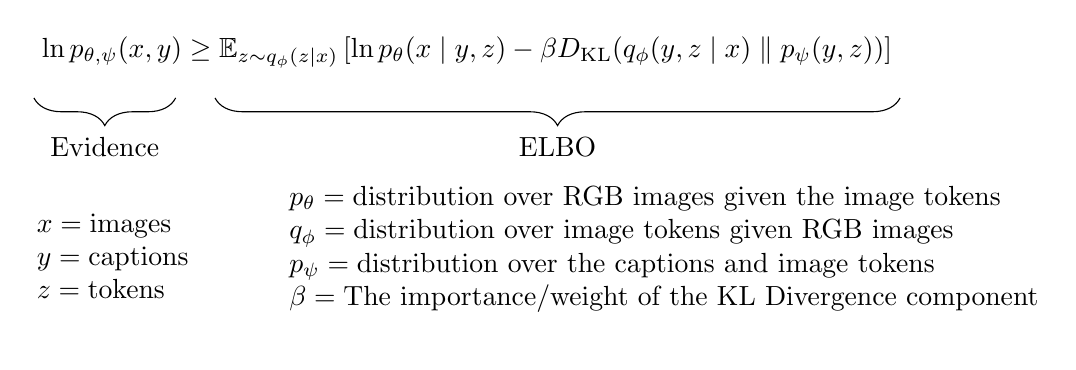
\begin{tikzpicture}
    \node at (0, 0) {$\ln p_{\theta, \psi}(x, y) \geq \mathbb{E}_{z \sim q_{\phi}(z|x)} \left[ \ln p_{\theta}(x \mid y, z) - \beta D_{\text{KL}}(q_{\phi}(y, z \mid x) \parallel p_{\psi}(y, z)) \right]$};


    % Draw curly braces and labels
    \draw [decorate,decoration={brace,amplitude=10pt,mirror,raise=5pt},yshift=0pt] (-5.5,-0.4) -- (-3.7, -0.4) node [black,midway,yshift=-0.8cm] {Evidence};
    \draw [decorate,decoration={brace,amplitude=10pt,mirror,raise=5pt},yshift=0pt] (-3.2, -0.4) -- (5.5, -0.4) node [black,midway,yshift=-0.8cm] {ELBO};

    \node[align=left] at (-4.5, -2.8) {
    $x = \text{images}$ \\
    $y = \text{captions}$ \\
    $z = \text{tokens}$ \\
    };

    % Add text descriptions for variables
    \node[align=left] at (2.5, -2.5) {
    $p_{\theta} = \text{distribution over RGB images given the image tokens}$ \\
    $q_{\phi} = \text{distribution over image tokens given RGB images}$ \\
    $p_{\psi} = \text{distribution over the captions and image tokens}$ \\
    $\beta = \text{The importance/weight of the KL Divergence component}$
    };
\end{tikzpicture}
\end{figure}

The first part, being the reconstruction loss, measures how accurately the dVAE decoder can reconstruct the image from its encoded latent variables. The second part, being the KL divergence, measures the distance between the learned posterior distribution to the prior distribution. \\

\begin{figure}[H]
    \centering
    \includegraphics[width=1\linewidth]{0_yosQ9u0cmtipniHZ.jpeg}
    \caption{The dVAE architecture (DALL-E Stage 1) [8]}
    \label{fig:enter-label}
\end{figure}

\item \textbf{Stage 2 - Training the Transformer:} The transformer in this architecture is responsible for catching the relationship between the tokenized textual descriptions and the corresponding image tokens. The image tokens are obtained by the dVAE trained at Stage 1. The transformer tries to predict the sequence of image tokens based on the text. \\

The architecture of the transformer is similar to that of GPT-3, as seen in Figure 7. However, it is designed to process both the text and the image in a single sequence. This is done by a simple concatenation of the image tokens to the text tokens. The text is tokenized via a BPE tokenizer.

The aim is to maximize the likelihood of the sequence of image tokens, given the corresponding text tokens. Each token is predicted one by one, all conditioned on the previous token in the sequence. This is done by applying Self-Attention to the sequences.  \\ \\

The training loss is simply an autoregressive cross-entropy loss, aiming to minimize the difference between the autoregressively predicted tokens and the actual tokens at each step. It can be formulated as:

\[\mathcal{L}_{\text{AR}} = -\sum_{t=N + 1}^{T} \log p(x_t \mid x_{<t})\]
\begin{itemize}
    \item N denotes the number of tokens (256) used for the textual description.
    \item T denotes the number of tokens present in the sequence.
    \item t denotes the index of the current token.
\end{itemize}

\begin{figure}
    \centering
    \includegraphics[width=1\linewidth]{stage2.jpg}
    \caption{The transformer architecture (DALL-E Stage 2) [8]}
    \label{fig:enter-label}
\end{figure}

\subsubsection{Capabilities and Examples}
In this subsection, some of the capabilities and impressive sample results of DALL-E will be discussed. \\
DALL-E is an extremely important model in the field of Generative Models. It can effectively generate images from textual prompts, as well as learn zero-shot. It can seamlessly combine multiple concepts that in real life have no relevance whatsoever. 

\begin{figure} [H]
    \centering
    \includegraphics[width=1\linewidth]{dall_e_prompts.png}
    \caption{Some qualitative results of DALL-E. [8]}
    \label{fig:enter-label}
\end{figure}

\subsection{Stable Diffusion}
\subsubsection{Model Architecture and Diffusion Process}
The main contribution of this model is the Latent Diffusion Model. The model effectively applies diffusion-based generation in a latent space, rather than the pixel space. This way, not only is the computational cost significantly lower, but the model also learns to work only on the parts that truly matter. 

The architecture, again, can be viewed in two steps:

\item \textbf{Latent Space Autoencoder:} In order to successfully map an input image to a latent space and back, we need to train an autoencoder, just like we did in DALL-E. The \textbf{encoder} should compress the input image into a lower-dimensional latent representation. This is achieved using ResNet blocks, and max-pooling layers for downsampling.
The \textbf{decoder} reconstructs the image from the latent representation, using ResNet blocks with nearest-neighbor upsampling. \\

The autoencoder is trained with a combination of perceptual loss and a patch-based adversarial objective to ensure that the reconstructions have high local realism.

The loss function consists of a perceptual loss, the difference between the original and the reconstructed image, and an adversarial loss, a GAN-inspired loss that improves realism by making the generated images indistinguishable from the real ones. 

\[\mathcal{L}_{\text{total}} = \mathcal{L}_{\text{perceptual}} + \lambda_{adv} \mathcal{L}_{\text{adversarial}}\]

\item \textbf{UNet Backbone:} The main part of this model is the UNet Backbone that works in the latent space.

\textbf{Diffusion Models:} The purpose of the diffusion models is to learn a data distribution, p(x), by gradually denoising a normal distribution variable. Essentially, in the forward process, noise is added step by step to eventually get to a normal distribution. By the Central Limit Theorem, if a distribution has converged to being a normal distribution after a noise addition of T steps, it will still be a normal distribution after step T + 1. \\

The gradual noise addition process, called the \textbf{Forward Process}, is as follows:
\[q(x_t | x_{t-1}) = \mathcal{N}(x_t; \sqrt{1 - \beta_t} x_t, \beta_t \mathbf{I})\]

where
\item $\hspace{50pt}$ $x_0$ is the original data sample.
\item $\hspace{50pt}$ $x_t$ is the data sample at timestamp t.
\item $\hspace{50pt}$ $\beta_t$ is the noise variance schedule.
\item $\hspace{50pt}$ $\mathcal{N}$ denotes the normal distribution. \\

One can efficiently sample $x_t$ from $x_0$ in t steps in the forward process without iterating through each timestamp using

\[q(x_t | x_0) = \mathcal{N}(x_t; \sqrt{\bar{\alpha}_t} x_0, (1 - \bar{\alpha}_t) \mathbf{I})\]

where \( \hspace{25pt} \bar{\alpha}_t = \prod_{s=1}^{t} (1 - \beta_s) \). \\

In the \textbf{backward process}, the goal is to remove the noise added in the forward process, effectively sampling data from the original distribution, or \textbf{generating new data}. To achieve this, a neural network is trained to predict the noise at each step. 

\[p_\theta(x_{t-1} | x_t) = \mathcal{N}(x_{t-1}; \mu_\theta(x_t, t), \sigma^2_t \mathbf{I})\]

The mean \(\mu_\theta(x_t, t)\) is predicted by a neural network parameterized by \(\theta\), and \(\sigma_t\) can be either fixed or learned.

The training objective for the backward process is:
\[L_{\text{simple}} = \mathbb{E}_{t, x_0, \epsilon} \left[ \|\epsilon - \epsilon_\theta(x_t, t) \|^2 \right]\]

where \( x_t = \sqrt{\bar{\alpha}_t} x_0 + \sqrt{1 - \bar{\alpha}_t} \epsilon \) and \(\epsilon \sim \mathcal{N}(0, \mathbf{I})\).

In the paper, however, the diffusion process is done on the latent space.

\begin{equation}
L_{\text{LDM}} := \mathbb{E}_{\mathcal{E}(x), \epsilon \sim \mathcal{N}(0,1), t} \left[ \left\| \epsilon - \epsilon_{\theta}(z_t, t) \right\|^2_2 \right]
\end{equation}

Samples from p(x) can be efficiently decoded into the latent space using the decoder. The neural backbone $\epsilon_{\theta}(\circ, t)$ is a time-conditional UNet structure. This backbone works in the latent space to carry out the denoising process. \\

\begin{figure}
    \centering
    \includegraphics[width=0.75\linewidth]{sd_unet_backbone.png}
    \caption{The architecture of the UNet Backbone in Stable Diffusion [9]}
    \label{fig:enter-label}
\end{figure}

The UNet backbone, whose architecture can be seen in Figure 9, contains cross-attention layers. These cross-attention layers provide conditioning when generating images. This cross-attention is done to suffice the $\epsilon_{\theta}(\circ, t, y)$ conditioning, where y is a condition from potentially a different modality (text, for our concern). Here, the conditions are in the form of an intermediate representation $\tau_\theta(y)$. Generally, CLIP text embedding is used to represent the text.\\


\[\text{Attention}(Q, K, V) = \text{softmax} \left( \frac{QK^T}{\sqrt{d}} \right) \cdot V\]
with
\[Q = W_Q \cdot \varphi_i(z_t), \quad K = W_K \cdot \tau_\theta(y), \quad V = W_V \cdot \tau_\theta(y).\]

Here, \(\varphi_i(z_t) \in \mathbb{R}^{N \times d_\epsilon^i}\) denotes a (flattened) intermediate representation of the UNet implementing \(\epsilon_\theta\) and W's are the learnable projection matrices of the (cross) attention mechanism.


\subsubsection{Capabilities and Examples}
Utilizing its architecture, Stable Diffusion can carry out the following tasks:
\item \textbf{Unconditional Image Generation} \\
\item \textbf{Conditional (for example, Text-to-) Image Generation:} Thanks to the cross-attention layers in the UNet backbone, Stable Diffusion manages to generate images based on conditions from different modalities. \\
\item \textbf{Image Impainting:} Stable Diffusion is very successful at filling the missing parts of an image, object removal for example. You can find an example of object removal using Stable Diffusion in Figure 10. \\

\item \textbf{Upsampling:} Stable Diffusion can upsample a given image using its decoder.

\begin{figure} [H]
    \centering
    \includegraphics[width=0.92\linewidth]{stable_diffusion_prompts.png}
    \caption{Conditional Image Generation using Stable Diffusion [9]}
    \label{fig:enter-label}
\end{figure}
\newpage
\section{References}
$\hspace{35pt}$ [1] Anderson, P., He, X., Buehler, C., Teney, D., Johnson, M., Gould, S., \& Zhang, L. (2017). Bottom-Up and Top-Down Attention for Image Captioning and Visual Question Answering. ArXiv. /abs/1707.07998 \\ \\

$\hspace{20pt}$ [2] Devlin, J., Chang, M., Lee, K., \& Toutanova, K. (2018). BERT: Pre-training of Deep Bidirectional Transformers for Language Understanding. ArXiv. /abs/1810.04805 \\ \\

$\hspace{20pt}$ [3] Gheini, M., Ren, X., \& May, J. (2021). Cross-Attention is All You Need: Adapting Pretrained Transformers for Machine Translation. ArXiv. /abs/2104.08771 \\ \\

$\hspace{20pt}$ [4] Lu, J., Batra, D., Parikh, D., \& Lee, S. (2019). ViLBERT: Pretraining Task-Agnostic Visiolinguistic Representations for Vision-and-Language Tasks. ArXiv. /abs/1908.02265 \\ \\

$\hspace{20pt}$ [5] Lu, J., Yang, J., Batra, D., \& Parikh, D. (2016). Hierarchical Question-Image Co-Attention for Visual Question Answering. ArXiv. /abs/1606.00061 \\ \\

$\hspace{20pt}$ [6] N, K. D. (2021). Using Large Pre-Trained Models with Cross-Modal Attention for Multi-Modal Emotion Recognition. ArXiv. /abs/2108.09669 \\

$\hspace{20pt}$ [7] Radford, A., Kim, J. W., Hallacy, C., Ramesh, A., Goh, G., Agarwal, S., Sastry, G., Askell, A., Mishkin, P., Clark, J., Krueger, G., \& Sutskever, I. (2021). Learning Transferable Visual Models From Natural Language Supervision. ArXiv. /abs/2103.00020 \\  \\

$\hspace{20pt}$ [8] Ramesh, A., Pavlov, M., Goh, G., Gray, S., Voss, C., Radford, A., Chen, M., \& Sutskever, I. (2021). Zero-Shot Text-to-Image Generation. ArXiv. /abs/2102.12092 \\ \\

$\hspace{20pt}$ [9] Rombach, R., Blattmann, A., Lorenz, D., Esser, P., \& Ommer, B. (2021). High-Resolution Image Synthesis with Latent Diffusion Models. ArXiv. /abs/2112.10752 \\ \\

$\hspace{20pt}$ [10] TensorFlow, "Word embeddings". Available at: \ https://www.tensorflow.org/text/guide/word\_embeddings [Accessed: 2024-06-18]. \\

$\hspace{20pt}$ [11] Xu, K., Ba, J., Kiros, R., Cho, K., Courville, A., Salakhutdinov, R., Zemel, R., \& Bengio, Y. (2015). Show, Attend and Tell: Neural Image Caption Generation with Visual Attention. ArXiv. /abs/1502.03044 \\ \\

$\hspace{20pt}$ [12] Zain ul Abideen, "How OpenAI’s DALL-E works?", Medium, 2021. Available at: \\https://medium.com/@zaiinn440/how-openais-dall-e-works-da24ac6c12fa [Accessed: 2024-06-18].
\end{document}
